%%%%%%%%%%%%%%%%%%%%%%%%%%%%%%%%%%%%%%%%%%%%%%%%%%%%%%%%%%%%%%%%%%%%%%%%%%%%%%%
% Definici\'on del tipo de documento.                                           %
% Posibles tipos de papel: a4paper, letterpaper, legalpapper                  %
% Posibles tama�os de letra: 10pt, 11pt, 12pt                                 %
% Posibles clases de documentos: article, report, book, slides                %
%%%%%%%%%%%%%%%%%%%%%%%%%%%%%%%%%%%%%%%%%%%%%%%%%%%%%%%%%%%%%%%%%%%%%%%%%%%%%%%
\documentclass[a4paper,10pt]{article}


%%%%%%%%%%%%%%%%%%%%%%%%%%%%%%%%%%%%%%%%%%%%%%%%%%%%%%%%%%%%%%%%%%%%%%%%%%%%%%%
% Los paquetes permiten ampliar las capacidades de LaTeX.                     %
%%%%%%%%%%%%%%%%%%%%%%%%%%%%%%%%%%%%%%%%%%%%%%%%%%%%%%%%%%%%%%%%%%%%%%%%%%%%%%%

% Paquete para inclusi\'on de gr\'aficos.
\usepackage{graphicx}

% Paquete para definir la codificaci\'on del conjunto de caracteres usado
% (latin1 es ISO 8859-1).
\usepackage[latin1]{inputenc}

% Paquete para definir el idioma usado.
\usepackage[spanish]{babel}

\usepackage{multirow} 

% Paquete para f\'ormulas matem\'aticas
\usepackage{amsmath}
\newcommand{\BigO}[1]{\ensuremath{\operatorname{O}\bigl(#1\bigr)}}

%\usepackage{multicolumn} 

% T\'itulo principal del documento.
\title{		\textbf{Trabajo pr\'actico 0: Infraestructura b\'asica}}

% Informaci\'on sobre los autores.
\author{	Alejandro Garc\'ia Marra, \textit{Padr\'on Nro. 91.516}                     \\
            \texttt{ alemarra@gmail.com }                                              \\
            Sebasti\'an Javier Bogado, \textit{Padr\'on Nro. 91.707}                     \\
            \texttt{ sebastian.j.bogado@gmail.com }                                              \\
            \normalsize{Grupo Nro. 0 - 2do. Cuatrimestre de 2012}                       \\
            \normalsize{66.20 Organizaci\'on de Computadoras}                             \\
            \normalsize{Facultad de Ingenier\'ia, Universidad de Buenos Aires}            \\
       }
\date{}



\begin{document}

% Inserta el t\'itulo.
\maketitle

% Quita el n\'umero en la primer p\'agina.
\thispagestyle{empty}

% Resumen
\begin{abstract}

\end{abstract}

\newpage
\section{Introducci\'on}

Muchas veces tanto para programas reci\'en terminados, como para aquellos que llevan un tiempo en funcionamiento, se desconoce realmente qu\'e partes del programa insumen la mayor cantidad de recursos, sean estos de tiempo, carga de cpu, etc.
Poseer esta informaci\'on se torna en algo cr\'itico cuando se busca realizar una mejora de performance en dicho programa. Ser\'ia poco \'util intentar optimizar a ciegas, por no decir in\'util.\\
Haremos uso entonces de tres herramientas distintas, el profiling del c\'odigo (por medio de \textit{gprof} y \texit{cachegrind}) y la medici\'on de los tiempos de ejecuci\'on (por medio de \textit{time}). 

\begin{itemize}
 \item \textbf{Profiling}: 

\begin{itemize}
	
\item {\textbf{gprof:} } {El profiling permite aprender donde el programa pasa la mayor parte de su tiempo, y cuales funciones llaman a otras mientras se ejecuta.\\
 			   Esta informacion puede mostrar qu\'e piezas del programa son mas lentas de lo esperado, convirti\'endolas en candidatas para su reescritura en la etapa de optimizaci\'on.\\
 			   Tambi\'en puede ayudarnos a descubrir cuales funciones son llamadas m\'as o menos veces delo esperado, pudiendo as\'i encontrar nuevos bugs (aunque el descubrimiento de bugs no es el fin principal de esta etapa)
 			   
			   El profiler utiliza informaci\'on recolectada en tiempo de ejecuci\'on, por lo que puede ser utilizado en programas demasiado grandes o complejos, donde un an\'alisis por lectura de fuentes ser\'ia impracticable.\\
			   Como consecuencia del an\'alisis durante la ejecuci\'on, los datos con los que se corra el programa afectaran el resultado del profiler. 
			   Es decir, distintos datos de entrada pueden provocar distintas ramas de ejecuci\'on, dando por resultado que, por ejemplo, no se llamen algunas funciones.}

\item{\textbf{CacheGrind:}}{}
			
\end{itemize}
			   
\item \textbf{Medici\'on de Tiempos}: Permite conocer con precisi\'on los tiempos de ejecuci\'on de un programa, discriminados entre tiempos de systema, de usario, tiempos totales, etc., as\'i como tambi\'en conocer los porcentajes para cada parte del programa, cantidad de entradas, y muchas otras opciones.\\
				     La combinaci\'on con una herramienta de profiling permite exactitud a la hora de conocer la forma en que se ejecuta el programa bajo estudio, permitiendo optimizar \'unicamente las partes cr\'iticas del ciclo de ejecuci\'on.
\end{itemize}


\newpage


\section{Flujo del programa}


\section{Mediciones}

\subsection{Valores Obtenidos}

En la tabla~\ref{tab001} se presentan las mediciones realizadas con \textbf{time} sobre ambos algoritmos de ordenamiento y con archivos de distintos tama�os.\\

Adem\'as de los archivos indicados en el enunciado, fueron agregadas mediciones sobre archivos con tama�os arbitrarios, mayores, con el fin de mostrar de mejor manera las diferencias entre algoritmos.

\begin{table}[!htp]
\begin{center}
\begin{tabular}{cc|c|c|c|c|c|c|} 
\cline{3-8}
& & \multicolumn{3}{ c|}{Quicksort} & \multicolumn{3}{c|}{Stooge sort}\\ \cline{3-8}
&   & Ordenado & Invertido & Aleatorio & Ordenado & Invertido & Aleatorio \\ \cline{1-8}
\multicolumn{1}{|c}{\multirow{3}{*}{1kb}} &
\multicolumn{1}{|c|}{real$^{*}$} & 0.00 & 0.00 &0.00 & 0.00 & 0.00 & 0.00 \\ \cline{2-8}
\multicolumn{1}{|c}{}                        &
\multicolumn{1}{|c|}{user$^{*}$} & 0.00 & 0.00 &0.00 & 0.00 & 0.00 & 0.00 \\ \cline{2-8}
\multicolumn{1}{|c}{}                        &
\multicolumn{1}{|c|}{sys$^{*}$} & 0.00 & 0.00 &0.00 & 0.00 & 0.00 & 0.00 \\ \cline{1-8}
\multicolumn{1}{|c}{\multirow{3}{*}{8kb}} &
\multicolumn{1}{|c|}{real} & 0.00 & 0.00 &0.00 & 0.02 & 0.02 & 0.01 \\ \cline{2-8}
\multicolumn{1}{|c}{}                        &
\multicolumn{1}{|c|}{user} & 0.00 & 0.00 &0.00 & 0.01 & 0.01 & 0.01 \\ \cline{2-8}
\multicolumn{1}{|c}{}                        &
\multicolumn{1}{|c|}{sys} & 0.00 & 0.00 &0.00 & 0.00 & 0.00 & 0.00 \\ \cline{1-8}
\multicolumn{1}{|c}{\multirow{3}{*}{16kb}} &
\multicolumn{1}{|c|}{real} & 0.00 & 0.00 &0.00 & 0.00 & 0.02 & 0.02 \\ \cline{2-8}
\multicolumn{1}{|c}{}                        &
\multicolumn{1}{|c|}{user} & 0.00 & 0.00 &0.00 & 0.00 & 0.01 & 0.02 \\ \cline{2-8}
\multicolumn{1}{|c}{}                        &
\multicolumn{1}{|c|}{sys} & 0.00 & 0.00 &0.00 & 0.00 & 0.00 & 0.00 \\ \cline{1-8}
\multicolumn{1}{|c}{\multirow{3}{*}{32kb}} &
\multicolumn{1}{|c|}{real} & 0.00 & 0.00 &0.00 & 0.17 & 0.17 & 0.17 \\ \cline{2-8}
\multicolumn{1}{|c}{}                        &
\multicolumn{1}{|c|}{user} & 0.00 & 0.00 &0.00 & 0.17 & 0.17 & 0.17 \\ \cline{2-8}
\multicolumn{1}{|c}{}                        &
\multicolumn{1}{|c|}{sys} & 0.00 & 0.00 &0.00 & 0.00 & 0.00 & 0.00 \\ \cline{1-8}
\multicolumn{1}{|c}{\multirow{3}{*}{64kb}} &
\multicolumn{1}{|c|}{real} & 0.00 & 0.00 &0.00 & 1.44 & 1.44 & 1.44 \\ \cline{2-8}
\multicolumn{1}{|c}{}                        &
\multicolumn{1}{|c|}{user} & 0.00 & 0.00 &0.00 & 1.44 & 1.43 & 1.44 \\ \cline{2-8}
\multicolumn{1}{|c}{}                        &
\multicolumn{1}{|c|}{sys} & 0.00 & 0.00 &0.00 & 0.00 & 0.00 & 0.00 \\ \cline{1-8}
\multicolumn{1}{|c}{\multirow{3}{*}{1024kb}} &
\multicolumn{1}{|c|}{real} & 0.04 & 0.03 &0.03 & $>$1500 & $>$1500 & $>$1500 \\ \cline{2-8}
\multicolumn{1}{|c}{}                        &
\multicolumn{1}{|c|}{user} & 0.03 & 0.02 &0.03 & $>$1500 & $>$1500 & $>$1500 \\ \cline{2-8}
\multicolumn{1}{|c}{}                        &
\multicolumn{1}{|c|}{sys} & 0.00 & 0.00 &0.00 & 0.00 & 0.00 & 0.00 \\ \cline{1-8}
\end{tabular}
\caption{Resultados comando Time } \label{tab001}
\end{center}
\end{table}

$^{*}$ Referencia: 
\begin{itemize}
 \item real: \%e, tiempo total real usado por el proceso.
 \item user: \%U, total de segundos-CPU usados por el proceso directamente.
 \item sys : \%S, total de segundos-CPU utilizados por el systema en nombre del proceso.
\end{itemize}



\subsection{An\'alisis de los datos}

La marcada diferencia entre la complejidad de los algoritmos se refleja en muestras tan chicas como la de 8kb. 
A partir de ah\'i, el Stooge sort ya hace suficiente uso del procesador como para ser notado por time, mientras que el Quicksort hace lo propio reci\'en en la muestra m\'as grande, de 1024kb. En este caso, el Stooge sort se torn\'o intolerable.

En la figura se muestra el gr\'afico del tiempo insumido por el Stooge sort para las distintas muestras, a excepci\'on de la de 1024kb, porque demanda una escala que har\'ia inapreciable la situaci\'on de las otras muestras.


\begin{figure}[!htp]
\begin{center}
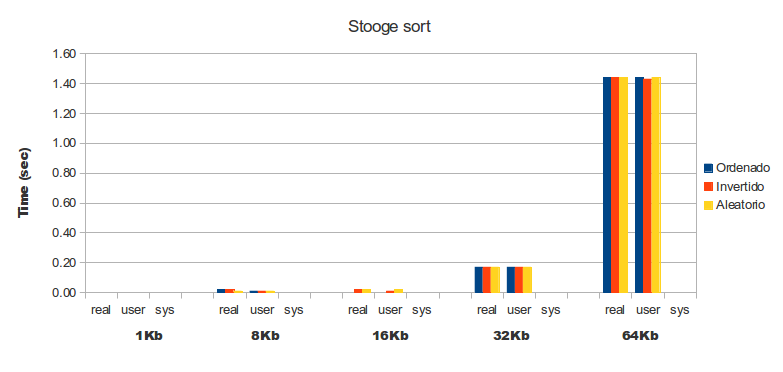
\includegraphics[width=1.1\textwidth]{stoogesort.png}
\end{center}
\caption{.} \label{fig002}
\end{figure}


Al momento de calcular el speedup de Quicksort contra Stooge sort, con la raz\'on entre los tiempos de cada uno, las cifras obtenidas no lo permiten. El primero no arroja resultados apreciables por \textbf{time} en ninguna instancia sin contar la \'ultima, donde el Stooge sort es inmanejable.\\

Esto es porque la complejidad del Quicksort es, en promedio, \BigO{n \log(n)}, mientras que el Stooge sort es de \BigO{n^{2,7}}. Entonces, el speedup entre ambos algoritmos tiende a infinito exponencialmente, seg\'un crece el tama�o de la muestra.


\section{Profiling}

Como se pudo apreciar en la tabla de tiempos de la p\'agina anterior, el algoritmo de quicksort resulta extremadamente veloz para tama�os de archivos relativamente grandes. Decidimos, entonces, forzar un poco m\'as al programa y hacer el profiling sobre un archivo desordenado de 32mb. Adem\'as, para que las funciones mismas de \textbf{gprof} tuvieran una incidencia despreciable en la prueba.\\
Realizar esta misma prueba sobre el algoritmo Stooge sort, ser\'ia impracticable, ya que los tiempos demandados ser\'ian demasiado grandes.

Un punto interesante a destacar son llamadas a m\'etodos de ordenamiento: como era de esperarse, no se realizan llamadas al m\'etodo stoogesort, lo cual confirma que el algoritmo no es utilizado.
										
										   Por otra parte, para el m\'etodo quicksort\_r que implementa dicho algoritmo, tenemos cientos de miles de llamados. Esto era de esperarse debido a las dimensiones del archivo y la naturaleza recursiva del algoritmo utilizado.

La tabla~\ref{tab002} es la salida del \textbf{gprof}, en particular aquella conocida como "flat profile". Muestra el uso de las funciones invocadas, ordenadas de mayor a menor seg\'un el porcentaje de tiempo de ejecuci\'on de cada una.

\begin{table}[!htp]
\begin{center}
\begin{tabular}{|r|r|r|r|r|r|r|}
\hline
	\%		&	cumulative  &	self	&			&	self	&	total	& \\
\hline          
	time	&	seconds		&	seconds	&	calls	&	s/call	&	s/call	&	name \\    
\hline
 	91.87	&	1.53		&	1.53	&	448399	&	0.00	&	 0.00	&	particionar \\
\hline
	2.40	&	1.57		&	0.04	&	448801	&	0.00	&	0.00	&	cargarBuffer \\
\hline
	1.80	&	1.60		&	0.03	&	3565398	&	0.00	&	0.00	&	swap \\
\hline
	1.80	&	1.63		&	0.03	&	1		&	0.03	&	0.07	&	parseLineas \\
\hline
	1.80	&	1.66		&	0.03	&	1		&	0.03	&	1.67	&	sort \\
\hline
	0.60	&	1.67		&	0.01	&	1		&	0.01	&	1.57	&	quickSort\_r \\
\hline
	0.00	&	1.67		&	0.00	&	1		&	0.00	&	0.00	&	check\_param \\
\hline
	0.00	&	1.67		&	0.00	&	1		&	0.00	&	1.57	&	quick\_sort \\
\hline
\end{tabular}
\caption{Ejemplo de tabla.} \label{tab002}
\end{center}
\end{table}
 
Se aprecia en la tabla que la funci\'on particionar ocupa el 91,87\% del tiempo de ejecuci\'on de programa, convirti\'endola en la candidata para mejorar.\par
\medskip
Para calcular el speedup m\'aximo, usamos la f\'ormula:

\begin{center}
$ speedup total = 1/(1-f + f/SM)$\\
\vspace{0.5cm}
$ f = 0,9187 $; SM tiende a infinito por ser arbitrariamente mejorable\\

\vspace{0.5cm}

$ Speedup maximo = 1/0,08123 = 12,3$
\end{center}


\newpage

\section{Comandos de ejecuci\'on y corridas de prueba}

Comandos de Compilaci\'on:

\begin{itemize}
 \item make all: genera el programa, modo release"
 \item make debug: genera el programa con flags para debugging
 \item make gprof: genera el programa con flags para \textbf{gprof}
 \item make clean: remueve los archivos generados
\end{itemize}

Comandos de Ejecuci\'on:

\begin{itemize}
\end{itemize}



\section{Conclusiones}

% Citas bibliogr\'aficas.
\begin{thebibliography}{99}


\end{thebibliography}

\end{document}
